% Archivo generado automáticamente por knapsack.c
\documentclass[12pt]{article}
\usepackage[utf8]{inputenc}
\usepackage{graphicx}
\usepackage{array,booktabs}
\usepackage[table]{xcolor}
\usepackage{longtable}
\usepackage{geometry}
\usepackage{pdflscape}
\usepackage{tikz}
\geometry{margin=0.8in}
\begin{document}
\begin{center}
{\large Instituto Tecnológico de Costa Rica\\[1cm]

\includegraphics[width=0.4\textwidth]{TEC.png}\\[2cm]
{\LARGE \textbf{Proyecto 3: Reemplazo de equipos}}\\[2cm]
{\large Investigación de Operaciones\\[2cm]
{\large Profesor: }\\[1cm]
{\large Francisco Jose Torres Roja}\\[2cm]
{\large Integrantes: }\\[1cm]
{\large Jose Pablo Fernandez Jimenez - 2023117752}\\[1cm]
{\large Diego Durán Rodríguez - 2022437509}\\[2cm]
{\large Segundo semestre 2025\\[1cm]
\end{center}
\newpage
\section*{Problema de Reemplazo de Equipos}
El \textbf{problema de reemplazo de equipos} es un problema clásico de toma de decisiones en investigación de operaciones. Consiste en determinar, a lo largo de un horizonte temporal, en qué momento resulta óptimo reemplazar un equipo (por ejemplo, una máquina, vehículo o computadora) considerando que, con el tiempo, su rendimiento disminuye y los costos de mantenimiento aumentan, mientras que su valor de reventa disminuye.

El objetivo es minimizar el costo total esperado. 

\textbf{Variantes del problema:}
\begin{itemize}
  \item \textit{Horizonte finito vs. infinito:} El análisis puede hacerse en un período limitado de tiempo o indefinido.
  \item \textit{Determinístico vs. estocástico:} En la versión determinística se conocen los costos y valores de reventa; en la estocástica, se modelan como variables aleatorias.
  \item \textit{Reemplazo individual vs. múltiple:} Puede plantearse para un único equipo o para varios equipos en paralelo.
\end{itemize}

\bigskip
\section*{Algoritmo utilizado}
El problema de reemplazo de equipos se resolvió utilizando la \textbf{ecuación recursiva de Bellman}, la cual permite determinar la decisión óptima en cada instante de tiempo aplicando el principio de optimalidad. 

La formulación es:

$$
G(t) = \min \{ C_{t,x} + G(x) \}
$$

donde:
\begin{itemize}
  \item $G(t)$ representa el costo mínimo óptimo a partir del instante $t$.
  \item $C_{t,x}$ es el costo de comprar el equipo en el instante $t$ y venderlo en el instante $x$.
  \item $G(x)$ corresponde a la decisión más óptima a partir del instante $x$.
\end{itemize}

De esta forma, en cada período se comparan las posibles decisiones (mantener el equipo o reemplazarlo) y se elige aquella que minimiza el costo total acumulado.

\bigskip
\section*{Problema}
\begin{itemize}
\item \textbf{Costo inicial del equipo:} 14000
\item \textbf{Plazo del proyecto:} 13 períodos
\item \textbf{Vida útil del equipo:} 5 períodos
\end{itemize}

\textbf{Datos iniciales de Reventa, Mantenimiento y ganancia:} 
\begin{table}[h!]
\centering
\begin{tabular}{|c|c|c|c|}
\hline
\textbf{Año de vida} & \textbf{Reventa} & \textbf{Mantenimiento} & \textbf{Ganancia} \\
\hline
1 & 6000 & 1500 & 0 \\
\hline
2 & 5500 & 1450 & 0 \\
\hline
3 & 5000 & 1000 & 0 \\
\hline
4 & 4700 & 1700 & 0 \\
\hline
5 & 4000 & 1500 & 0 \\
\hline
\end{tabular}
\end{table}

\newpage
\begin{landscape}
\subsection*{Costos de cada periodo $C_{t,x}$}
\begin{longtable}{|c|c|c|c|c|c|c|c|c|c|c|c|c|c|}
\hline
$t \to x$  & 1 & 2 & 3 & 4 & 5 & 6 & 7 & 8 & 9 & 10 & 11 & 12 & 13 \\\hline\hline
0 & 9500 & 11450 & 12950 & 14950 & 17150 & - & - & - & - & - & - & - & - \\\hline
1 & - & 9500 & 11450 & 12950 & 14950 & 17150 & - & - & - & - & - & - & - \\\hline
2 & - & - & 9500 & 11450 & 12950 & 14950 & 17150 & - & - & - & - & - & - \\\hline
3 & - & - & - & 9500 & 11450 & 12950 & 14950 & 17150 & - & - & - & - & - \\\hline
4 & - & - & - & - & 9500 & 11450 & 12950 & 14950 & 17150 & - & - & - & - \\\hline
5 & - & - & - & - & - & 9500 & 11450 & 12950 & 14950 & 17150 & - & - & - \\\hline
6 & - & - & - & - & - & - & 9500 & 11450 & 12950 & 14950 & 17150 & - & - \\\hline
7 & - & - & - & - & - & - & - & 9500 & 11450 & 12950 & 14950 & 17150 & - \\\hline
8 & - & - & - & - & - & - & - & - & 9500 & 11450 & 12950 & 14950 & 17150 \\\hline
9 & - & - & - & - & - & - & - & - & - & 9500 & 11450 & 12950 & 14950 \\\hline
10 & - & - & - & - & - & - & - & - & - & - & 9500 & 11450 & 12950 \\\hline
11 & - & - & - & - & - & - & - & - & - & - & - & 9500 & 11450 \\\hline
12 & - & - & - & - & - & - & - & - & - & - & - & - & 9500 \\\hline
\end{longtable}
\end{landscape}
\section*{Tabla de trabajo}
\begin{tabular}{ccc}\toprule
t & G(t) & Próximo \\\midrule
0 & 47050 & 4,5 \\
1 & 44850 & 5 \\
2 & 42850 & 5,6 \\
3 & 34300 & 8 \\
4 & 32100 & 8,9 \\
5 & 29900 & 9 \\
6 & 27900 & 9,10 \\
7 & 25900 & 10 \\
8 & 17150 & 13 \\
9 & 14950 & 13 \\
10 & 12950 & 13 \\
11 & 11450 & 13 \\
12 & 9500 & 13 \\
13 & 0 & - \\
\bottomrule\end{tabular}
\section*{Solución óptima}
Costo mínimo total: \textbf{47050} \\
\newpage
\begin{landscape}
\subsection*{Planes óptimos}
\begin{itemize}
  \item 0 - 4 - 8 - 13
\begin{center}
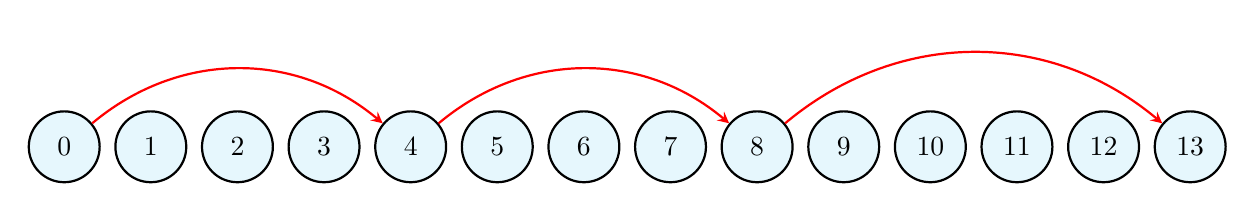
\begin{tikzpicture}[>=stealth,thick,scale=1.0]
\node[circle,draw,fill=cyan!10,minimum size=0.9cm] (n0) at (0.0,0) {0};
\node[circle,draw,fill=cyan!10,minimum size=0.9cm] (n1) at (1.1,0) {1};
\node[circle,draw,fill=cyan!10,minimum size=0.9cm] (n2) at (2.2,0) {2};
\node[circle,draw,fill=cyan!10,minimum size=0.9cm] (n3) at (3.3,0) {3};
\node[circle,draw,fill=cyan!10,minimum size=0.9cm] (n4) at (4.4,0) {4};
\node[circle,draw,fill=cyan!10,minimum size=0.9cm] (n5) at (5.5,0) {5};
\node[circle,draw,fill=cyan!10,minimum size=0.9cm] (n6) at (6.6,0) {6};
\node[circle,draw,fill=cyan!10,minimum size=0.9cm] (n7) at (7.7,0) {7};
\node[circle,draw,fill=cyan!10,minimum size=0.9cm] (n8) at (8.8,0) {8};
\node[circle,draw,fill=cyan!10,minimum size=0.9cm] (n9) at (9.9,0) {9};
\node[circle,draw,fill=cyan!10,minimum size=0.9cm] (n10) at (11.0,0) {10};
\node[circle,draw,fill=cyan!10,minimum size=0.9cm] (n11) at (12.1,0) {11};
\node[circle,draw,fill=cyan!10,minimum size=0.9cm] (n12) at (13.2,0) {12};
\node[circle,draw,fill=cyan!10,minimum size=0.9cm] (n13) at (14.3,0) {13};
\draw[->,thick,red,bend left=40] (n0) to (n4);
\draw[->,thick,red,bend left=40] (n4) to (n8);
\draw[->,thick,red,bend left=40] (n8) to (n13);
\end{tikzpicture}
\end{center}
  \item 0 - 4 - 9 - 13
\begin{center}
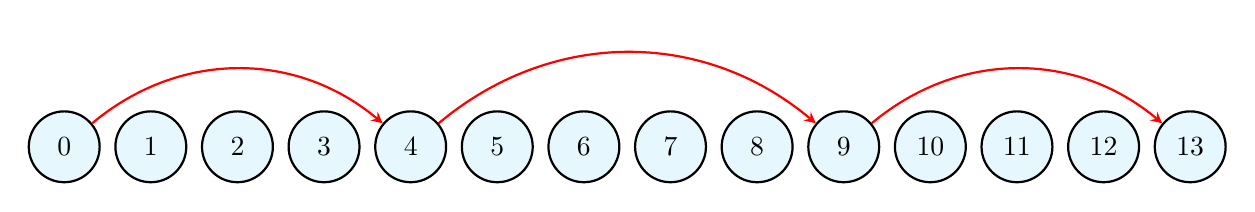
\begin{tikzpicture}[>=stealth,thick,scale=1.0]
\node[circle,draw,fill=cyan!10,minimum size=0.9cm] (n0) at (0.0,0) {0};
\node[circle,draw,fill=cyan!10,minimum size=0.9cm] (n1) at (1.1,0) {1};
\node[circle,draw,fill=cyan!10,minimum size=0.9cm] (n2) at (2.2,0) {2};
\node[circle,draw,fill=cyan!10,minimum size=0.9cm] (n3) at (3.3,0) {3};
\node[circle,draw,fill=cyan!10,minimum size=0.9cm] (n4) at (4.4,0) {4};
\node[circle,draw,fill=cyan!10,minimum size=0.9cm] (n5) at (5.5,0) {5};
\node[circle,draw,fill=cyan!10,minimum size=0.9cm] (n6) at (6.6,0) {6};
\node[circle,draw,fill=cyan!10,minimum size=0.9cm] (n7) at (7.7,0) {7};
\node[circle,draw,fill=cyan!10,minimum size=0.9cm] (n8) at (8.8,0) {8};
\node[circle,draw,fill=cyan!10,minimum size=0.9cm] (n9) at (9.9,0) {9};
\node[circle,draw,fill=cyan!10,minimum size=0.9cm] (n10) at (11.0,0) {10};
\node[circle,draw,fill=cyan!10,minimum size=0.9cm] (n11) at (12.1,0) {11};
\node[circle,draw,fill=cyan!10,minimum size=0.9cm] (n12) at (13.2,0) {12};
\node[circle,draw,fill=cyan!10,minimum size=0.9cm] (n13) at (14.3,0) {13};
\draw[->,thick,red,bend left=40] (n0) to (n4);
\draw[->,thick,red,bend left=40] (n4) to (n9);
\draw[->,thick,red,bend left=40] (n9) to (n13);
\end{tikzpicture}
\end{center}
  \item 0 - 5 - 9 - 13
\begin{center}
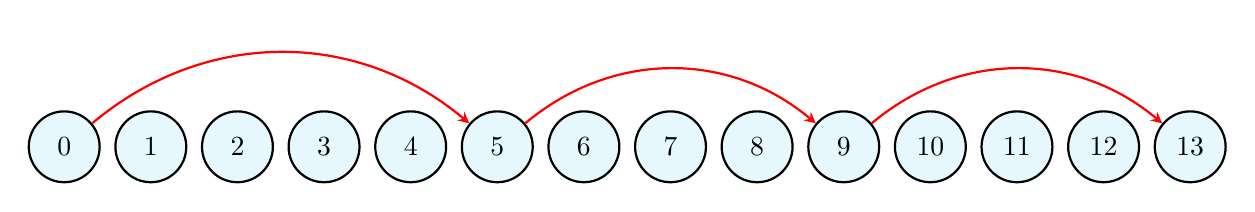
\begin{tikzpicture}[>=stealth,thick,scale=1.0]
\node[circle,draw,fill=cyan!10,minimum size=0.9cm] (n0) at (0.0,0) {0};
\node[circle,draw,fill=cyan!10,minimum size=0.9cm] (n1) at (1.1,0) {1};
\node[circle,draw,fill=cyan!10,minimum size=0.9cm] (n2) at (2.2,0) {2};
\node[circle,draw,fill=cyan!10,minimum size=0.9cm] (n3) at (3.3,0) {3};
\node[circle,draw,fill=cyan!10,minimum size=0.9cm] (n4) at (4.4,0) {4};
\node[circle,draw,fill=cyan!10,minimum size=0.9cm] (n5) at (5.5,0) {5};
\node[circle,draw,fill=cyan!10,minimum size=0.9cm] (n6) at (6.6,0) {6};
\node[circle,draw,fill=cyan!10,minimum size=0.9cm] (n7) at (7.7,0) {7};
\node[circle,draw,fill=cyan!10,minimum size=0.9cm] (n8) at (8.8,0) {8};
\node[circle,draw,fill=cyan!10,minimum size=0.9cm] (n9) at (9.9,0) {9};
\node[circle,draw,fill=cyan!10,minimum size=0.9cm] (n10) at (11.0,0) {10};
\node[circle,draw,fill=cyan!10,minimum size=0.9cm] (n11) at (12.1,0) {11};
\node[circle,draw,fill=cyan!10,minimum size=0.9cm] (n12) at (13.2,0) {12};
\node[circle,draw,fill=cyan!10,minimum size=0.9cm] (n13) at (14.3,0) {13};
\draw[->,thick,red,bend left=40] (n0) to (n5);
\draw[->,thick,red,bend left=40] (n5) to (n9);
\draw[->,thick,red,bend left=40] (n9) to (n13);
\end{tikzpicture}
\end{center}
\end{itemize}
\end{landscape}
\newpage
\begin{thebibliography}{9}
\bibitem{meyer1971} Meyer, R. A. (1971). Equipment replacement under uncertainty. \textit{Management Science, 17}(11), 750--758. https://doi.org/10.1287/mnsc.17.11.750

\bibitem{tan2010} Tan, C., \\& Hartman, J. (2010). Equipment replacement analysis with an uncertain finite horizon. Disponible en: https://econpapers.repec.org/article/tafuiiexx/v\_3a42\_3ay\_3a2010\_3ai\_3a5\_3ap\_3a342-353.htm

\end{thebibliography}
\end{document}
